\chapter{Исследовательская часть}

Технические характеристики устройства, на котором было произведено тестирование разработанного ПО: 

\begin{itemize}
	\item операционная система: macOS Big Sur 11.6.4;
	\item оперативная память: 8 Гб;
	\item 2,4 Ггц 2‑ядерный процессор Intel Core i5;
\end{itemize}

Во время тестирования ноутбук был включен в сеть питания.

\section{Время выполнения реализаций алгоритмов}

В таблицах \ref{tab:time1} -- \ref{tab:time3} представлены замеры времени работы для каждого из алгоритмов для отсортированных массивов, массивов из случайных чисел и неотсортированных массивов. Здесь и далее: БС — блочная сортировка, СП -- сортировка перемешиванием, СБД -- сортировка бинарным деревом. Высчитывалось среднее время в секундах работы алгоритмов при количестве повторений равном пятидесяти.

\begin{table}[h]
	\begin{center}
		\caption{\label{tab:time1}Результаты замеров времени алгоритмов на отсортированных массивах}
		\begin{tabular}{|c|c|c|c|c|}
		\hline
		Размер & БС &  СП & СБД \\
		\hline
		500  & 0.0033 & 0.0944 & 0.0458\\
		\hline
		750  & 0.0052 & 0.2581 & 0.1061\\
		\hline
		1000  & 0.0066 & 0.4021 & 0.2084 \\
		\hline
		1250  & 0.0098 & 0.6588 & 0.3221 \\
		\hline
		1500  & 0.0109 & 1.1394 & 0.4929 \\ 
		\hline
		1750  & 0.0116 & 1.3223 & 0.5063 \\
		\hline
		2000  & 0.0135 & 1.7849 & 0.8165 \\
		\hline
		\end{tabular}
	\end{center}
\end{table}

\begin{table}[h]
	\begin{center}
		\caption{\label{tab:time2}Результаты замеров времени алгоритмов на массивах из случайных чисел}
		\begin{tabular}{|c|c|c|c|c|}
		\hline
		Размер & БС &  СП & СБД \\
		\hline
		500  & 0.0069 & 0.1313 & 0.0021\\
		\hline
		750  & 0.0121 & 0.3305 & 0.0038\\
		\hline
		1000  & 0.0204 & 0.5272 & 0.0048\\
		\hline
		1250  & 0.0286 & 0.8101 & 0.0061\\
		\hline
		1500  & 0.0383 & 1.1723 & 0.0072\\ 
		\hline
		1750  & 0.0511 & 1.7372 &  0.0082\\
		\hline
		2000  & 0.0656 & 2.5861 & 0.0106 \\
		\hline
		\end{tabular}
	\end{center}
\end{table}

\begin{table}[h]
	\begin{center}
		\caption{\label{tab:time3}Результаты замеров времени алгоритмов на отсортированных в обратном порядке массивах}
		\begin{tabular}{|c|c|c|c|c|}
		\hline
		Размер & БС &  СП & СБД \\
		\hline
		500  & 0.0036 & 0.2136 & 0.1041\\
		\hline
		750  & 0.0051 & 0.5488 & 0.1399\\
		\hline
		1000  & 0.0099 & 0.8875 & 0.1849\\
		\hline
		1250  & 0.0081 & 1.2612 & 0.3215\\
		\hline
		1500  & 0.0103 & 1.6534 & 0.4063\\ 
		\hline
		1750  & 0.0117 & 2.3841 &  0.4865\\
		\hline
		2000  & 0.0135 & 2.7928 & 0.6994 \\
		\hline
		\end{tabular}
	\end{center}
\end{table}

На рисунке 4.4 изображены графики зависимости времени работы алгоритмов сортировок от количества элементов массивов. 

\begin{figure}[h!]
	\centering
	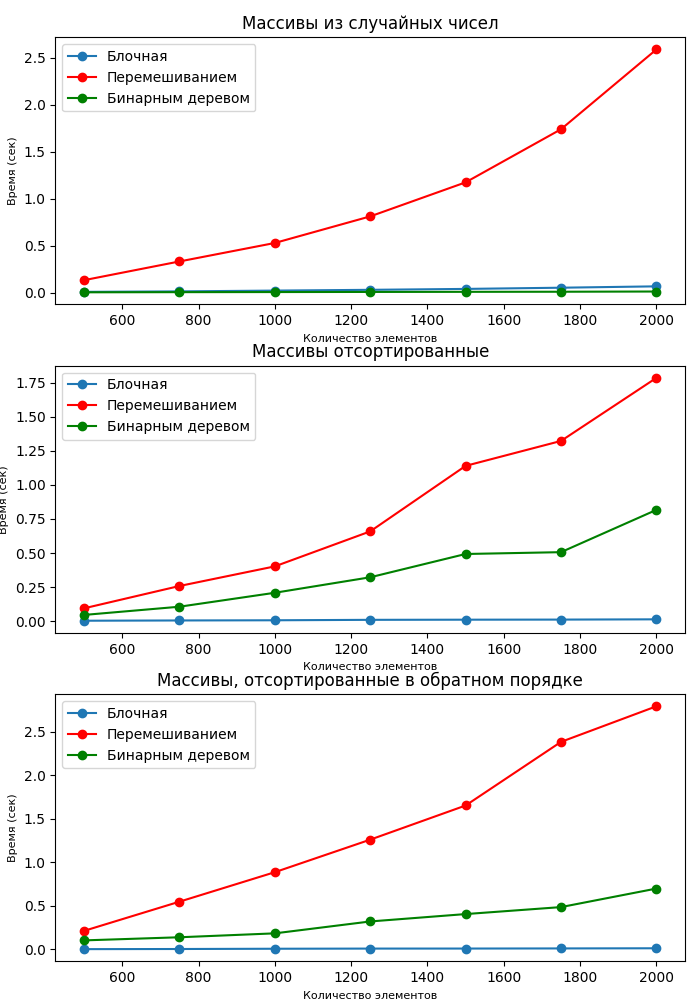
\includegraphics[width=1\linewidth]{img/Plot.png}
	\caption{Время работы сортировок}
	\label{fig:mpr}
\end{figure}


\section{Используемая память}

Пусть дан массив N элементов сравниваемого типа Type. Тогда затраты по памяти для алгоритмов будут следующие:

\begin{itemize}
\item блочная сортировка:\begin{itemize}
	\item длина массива, смещение -- $2 \cdot MemoryLayout<Int>.size$
	\item минимальный и максимальный элементы, размер блока -- $3 \cdot MemoryLayout<Type>.size$
	\item массив -- $N \cdot MemoryLayout<Type>.size$
\end{itemize}

\item сортировка перемешиванием:\begin{itemize}
	\item переменные right, left -- $2 \cdot MemoryLayout<Int>.size$
	\item массив -- $N \cdot MemoryLayout<Type>.size$
	\item переменная-буфер для обмена элементов местами -- 
	\newline $1 \cdot  MemoryLayout<Type>.size$
\end{itemize}

\item сортировка бинарным деревом:\begin{itemize}
	\item массив -- $N \cdot MemoryLayout<Type>.size$
	\item бинарное дерево -- $N \cdot (3 \cdot MemoryLayout<Type>.size)$
\end{itemize}
\end{itemize}

Нетрудно заметить, что самой затратной по памяти является сортировка бинарным деревом из-за необходимости хранить не только массив и несколько вспомогательных переменных, как в двух других реализациях сортировок, но и структуру бинарного дерева. Размеры же памяти, занимаемой сортировкой перемешиванием и блочной, разнятся не сильно. 

\end{itemize}
	
\section*{Вывод}
Экспериментально получено, что при любом наборе входных данных самой медленной оказывается сортировка перемешиванием, а самой независимой к характеристикам входных данных (отсортированный массив, неотсортированный массив, массив случайных чисел) является блочная сортировка. Использование реализации с бинарным деревом эффективно с массивом случайных чисел, однако ее показатели не разнятся при работе с отсортированными массивами и массивами, отсортированными в обратном порядке. В среднем для работы с массивами, состоящими из неупорядоченных данных, время работы бинарной и блочной сортировок практически не отличается и растет как линейная функция, а то время как сортировка перемешиванием уступает им в 1.5 раза и изменяется как функция квадратичная. Самой же неэффективной по памяти является сортировка бинарным деревом из-за необходимости хранить структуру бинарного дерева. 
